\documentclass{article}
\usepackage[utf8]{inputenc}
\usepackage{forest}
\usepackage{tikz}
\usepackage{subcaption}
\usepackage{caption}
\usepackage{amsmath}


\title{DARPA Heat Exchanger Model}
\author{Berk Ozturk, Ned Burnell, Bob Haimes}
\date{April 2018}

\begin{document}

\maketitle

\section{Introduction}

We use signomial programming (SP) to design a heat exchanger (HX) that takes advantage of the manufacturing capabilities of modern 3D printers. 

\section{Models}

\subsection{Levels of abstraction}
\label{ss:abstraction}

We can think of three levels of abstraction in a heat exchanger, which correspond directly to Python GPkit objects, which inherit the variables and constraints from the level below 

\begin{itemize}
    \item Cell level (\textbf{HXArea} object)
    \item Channel level (\textbf{RectPipe} object)
    \item Layer level (\textbf{Layer} object)
\end{itemize}

\begin{figure}
\centering
    \begin{forest}
        [\textbf{Layer}
            [\textbf{ColdPipe}
            [$N_{coldpipes}$]
            ]
            [\textbf{HXArea}
            [$N_{coldpipes} \times N_{hotpipes}$]            
            ]
            [\textbf{HotPipe}
            [$N_{hotpipes}$]
            ]
        ]
    \end{forest}
    \caption{\textnormal{Variable and constraint hierarchy in the SP HX formulation, with number of instances of each model in the leaf nodes.}}
    \label{f:hierarchyTree}
\end{figure}

\begin{center}
\begin{figure}
\centering
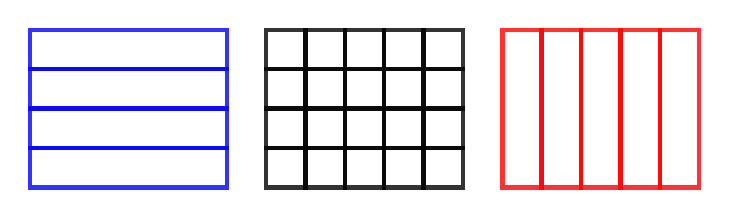
\begin{tikzpicture}[xscale=0.5,yscale=0.5]
\begin{scope}[thick,red]
  \foreach \x in {0,1,2,3,4}
  \draw[ultra thick,red,opacity=.8] (12+\x,0)rectangle(12+\x+1,4);
  
  \foreach \x in {0,1,2,3,4}
  \foreach \y in {0,1,2,3}
  \draw[ultra thick,black,opacity=.8] (6+\x,\y)rectangle(6+\x+1,\y+1);
  
  \foreach \y in {0,1,2,3}
  \draw[ultra thick, blue, opacity=0.8] (0, \y) rectangle (5,\y+1);
\end{scope}
\end{tikzpicture}
\caption{\textnormal{The corresponding geometric abstraction of the vectorized models, demonstrated for 4 cold and 5 hot pipes. Each cell corresponds to an instance of a GPkit model.}}
\end{figure}
\end{center}

\subsection{Partitioning models}

Within the framework described in Section~\ref{ss:abstraction}, we can partition the different types of heat transfer and flow models so that constraints are placed in models that contain and inherit all of the necessary variables. 

\subsubsection{\textbf{Pipe} model}

The \textbf{RectPipe} model defines the channel elements of the heat exchanger, and describes the fluid-wall interactions that result in a transfer of heat. 

\subsubsection{\textbf{HXArea} model}

The \textbf{HXArea} model 

It also defines the fluid-wall interface temperature, which differs from the internal temperature of the plate since there is thermal resistance through the plate which has to conduct the heat from one fluid to another. 

It also makes sure that the individual conductive members of the heat exchanger are not thinner than the minimum thicknesses allowed by a specific method of manufacturing. 

\begin{align}
    t_{plate} &\geq t_{min-material} /
    t_{hot}  &\geq t_{min-material} /
    t_{cold} &\geq t_{min-material} 
\end{align}

\subsection{Inputs to model}


However, different set of inputs can be used to converge the model as long as the unbounded variables described in \textbf{Layer} are appropriately bounded. 

\subsection{Objective}

Currently, the objective of the model is the inverse of the total heat transfer 

\subsection{Use cases for the model}

\begin{itemize}
    \item Experiment with different materials to see how the 
\end{itemize}

\subsection{Future work}

There is plenty to be done to improve the robustness of the optimization method and to generalize it to arbitrary cell tile shapes. 

\end{document}
